
\usetikzlibrary{decorations.pathmorphing,patterns,arrows.meta}

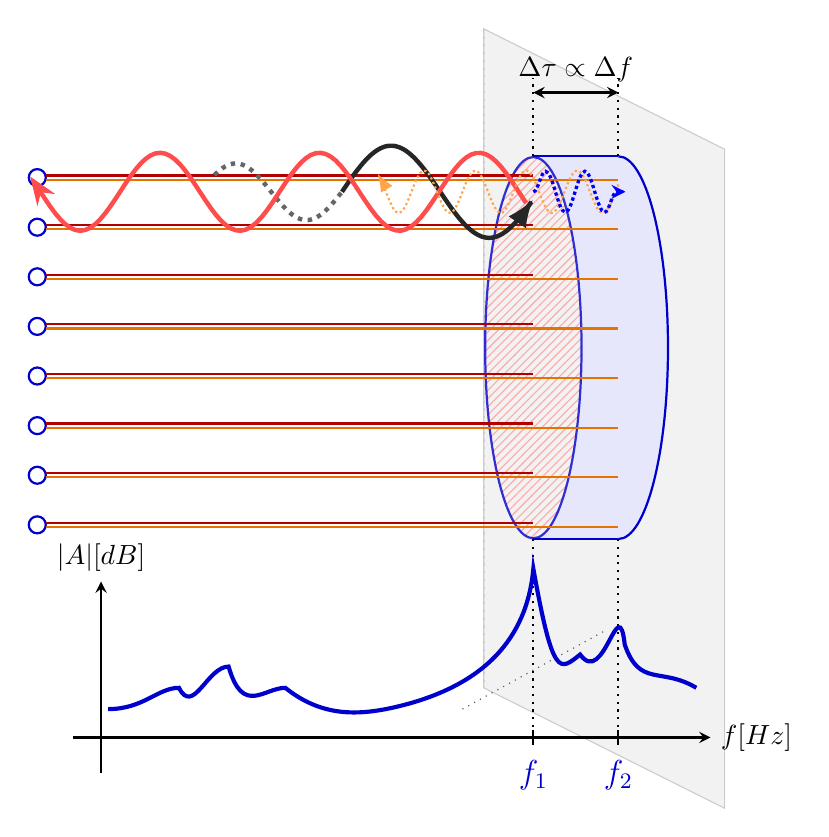
\begin{tikzpicture}[scale=0.9, >=stealth]

    % --- 1. CAPA DE FONDO: MARCO EN PERSPECTIVA ---
    \draw[gray!40, thin, fill=black!5] (0.8, 7.5) -- (4.2, 5.8) -- (4.2, -3.5) -- (0.8, -1.8) -- cycle;
    \draw[gray!40, dotted, thick] (0.8, 7.5) -- (0.8, -1.8);

    % --- 2. CAPA DE LA PASTILLA (Cuerpo y Relleno) ---

    \fill[blue!10, opacity=0.8]
        (1.5, 5.7) -- (2.7, 5.7)
        arc (90:-90:0.7cm and 2.7cm)
        -- (1.5, 0.3)
        arc (-90:90:0.7cm and 2.7cm)
        -- cycle;

    \draw[thick, blue!80!black]
        (2.7, 0.3) arc (-90:90:0.7cm and 2.7cm);

    \draw[thick, blue!80!black] (1.5, 5.7) -- (2.7, 5.7);
    \draw[thick, blue!80!black] (1.5, 0.3) -- (2.7, 0.3);

    \draw[
        thick,
        blue!80!black,
        fill=red!15,
        opacity=0.8,
        pattern=north east lines,
        pattern color=red!40
    ]
    (1.5, 3.0) ellipse[x radius=0.68cm, y radius=2.69cm];

    % --- 3. CAPA DE LÍNEAS INCIDENTES ---

    \foreach \y in {0.5,1.2,1.9,2.6,3.3,4.0,4.7,5.4}{
        \draw[thick, blue!80!black] (-5.5,\y) circle (0.12);
        \draw[thick, red!70!black] (-5.38,\y+0.03) -- (1.5,\y+0.03);
        \draw[thick, orange!90!black] (-5.38,\y-0.03) -- (2.7,\y-0.03);
    }

    % --- 4. CAPA DE ONDAS SUPERIORES ---

    \draw[dotted, ultra thick, black!60, samples=50, domain=-3.0:-1.2]
        plot (\x,{5.2 + 0.4*sin((\x+1.2)*180)});

    \draw[
        black!85,
        samples=100,
        domain=-1.2:1.5,
        arrows=-Latex,
        ultra thick
    ]
        plot (\x,{5.2 + 0.65*sin((\x+1.2)*130)});

    \draw[
        red!70,
        samples=100,
        domain=-5.6:1.4,
        arrows=Stealth-,
        ultra thick
    ]
        plot (\x,{5.2 + 0.55*sin((\x+1.8)*160 + 45)});

    \draw[
        thick,
        dash dot,
        samples=80,
        domain=2.7:-0.7,
        arrows=-Latex,
        densely dotted,
        orange!71
    ]
        plot (\x,{5.2 + 0.30*sin((\x+1.0)*500 - 30)});

    \draw[
        line width=1.2pt,
        blue,
        decorate,
        decoration={
            snake,
            segment length=7pt,
            amplitude=3.5pt
        },
        ->,
        densely dotted,
        /pgf/decoration/segment length=14.2pt,
        /pgf/decoration/amplitude=7.4pt
    ]
        (1.5,5.2) -- (2.8,5.2);

    % --- 5. CORTES Y COTAS DE MEDIDA ---

    \draw[dotted, thick] (1.5,5.7) -- (1.5,6.8);
    \draw[dotted, thick] (2.7,5.7) -- (2.7,6.8);

    \draw[<->, thick]
        (1.5,6.6) -- (2.7,6.6)
        node[midway,above]
        {$\Delta \tau \propto \Delta f$};

    \draw[dotted, thick] (1.5,0.3) -- (1.5,-2.4);
    \draw[dotted, thick] (2.7,0.3) -- (2.7,-2.4);

    % --- 6. GRÁFICA INFERIOR ---

    \draw[->, thick]
        (-5.0,-2.5) -- (4.0,-2.5)
        node[right] {$f[Hz]$};

    \draw[->, thick]
        (-4.6,-3.0) -- (-4.6,-0.3)
        node[above] {$|A|[\text{dB}]$};

    \draw[thick]
        (1.5,-2.4) -- (1.5,-2.6)
        node[below=2pt,blue!80!black] {\large $f_1$};

    \draw[thick]
        (2.7,-2.4) -- (2.7,-2.6)
        node[below=2pt,blue!80!black] {\large $f_2$};

    \draw[dotted, thin, black!70]
        (0.5,-2.1) -- (2.5,-1.0);

    \draw[line width=1.5pt, blue!80!black, smooth]
        (-4.5,-2.1)
        .. controls (-4.0,-2.1) and (-3.8,-1.8) .. (-3.5,-1.8)
        .. controls (-3.3,-2.2) and (-3.1,-1.5) .. (-2.8,-1.5)
        .. controls (-2.6,-2.2) and (-2.3,-1.8) .. (-2.0,-1.8)
        .. controls (-1.5,-2.2) and (-1.0,-2.2) .. (-0.44,-2.07)
        .. controls (0.8,-1.78) and (1.41,-1.11) .. (1.5,-0.12)
        .. controls (1.78,-1.68) and (1.87,-1.56) .. (2.16,-1.33)
        .. controls (2.5,-1.8) and (2.7,-0.4) .. (2.79,-1.19)
        .. controls (3.0,-1.8) and (3.3,-1.5) .. (3.8,-1.8);

\end{tikzpicture}

